
% v2-acmsmall-sample.tex, dated March 6 2012
% This is a sample file for ACM small trim journals
%
% Compilation using 'acmsmall.cls' - version 1.3 (March 2012), Aptara Inc.
% (c) 2010 Association for Computing Machinery (ACM)
%
% Questions/Suggestions/Feedback should be addressed to => "acmtexsupport@aptaracorp.com".
% Users can also go through the FAQs available on the journal's submission webpage.
%
% Steps to compile: latex, bibtex, latex latex
%
% For tracking purposes => this is v1.3 - March 2012
\documentclass[prodmode,acmtecs]{acmsmall} % Aptara syntax
\usepackage[spanish,polish]{babel}
\usepackage[T1]{fontenc}
\usepackage{fancyvrb}
\usepackage{graphicx,hyperref}
\newcommand\cutout[1]{}


\usepackage[table]{xcolor}
\usepackage[utf8]{inputenc}
\usepackage[parfill]{parskip}
\usepackage{tabulary}
\PassOptionsToPackage{hyphens}{url}
\usepackage{hyperref}    
\usepackage[capitalize]{cleveref}


% Metadata Information
% !!! TODO: SET THESE VALUES !!!
\acmVolume{0}
\acmNumber{0}
\acmArticle{CFP}
\acmYear{0}
\acmMonth{0}

\newcounter{colstart}
\setcounter{page}{4}

\RecustomVerbatimCommand{\VerbatimInput}{VerbatimInput}%
{
%fontsize=\footnotesize,
fontfamily=\rmdefault
}


\newcommand{\UnderscoreCommands}{%\do\verbatiminput%
\do\citeNP \do\citeA \do\citeANP \do\citeN \do\shortcite%
\do\shortciteNP \do\shortciteA \do\shortciteANP \do\shortciteN%
\do\citeyear \do\citeyearNP%
}

\usepackage[strings]{underscore}



% Document starts
\begin{document}


\setcounter{colstart}{\thepage}

\acmArticle{CFP}
\title{{\huge\sc SIGLOG Monthly 257}

 January 2025}\author{ELLI ANASTASIADI\affil{Aalborg University, SE}\vspace*{-2.6cm}\begin{flushright}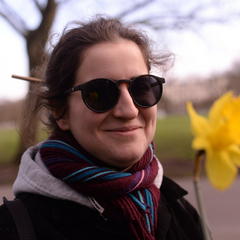
\includegraphics[width=30mm]{elli_anastasiadi.png}\end{flushright}}\begin{abstract}January 2025 edition of SIGLOG Monthly, featuring deadlines, calls and community announcements.
\end{abstract}


\maketitlee

\href{https://lics.siglog.org/newsletters/}{Past Issues}
 - 
\href{https://lics.siglog.org/newsletters/inst.html}{How to submit an announcement}
\section{Table of Contents}\begin{itemize}\item DEADLINES (\cref{deadlines}) 
 
\item CALLS 
 
\begin{itemize}\item LMW@CSL 2025 (CALL FOR PARTICIPATION - s SIGLOG MATTER) (\cref{LMWCSL2025})
\item ICGT 2025 (CALL FOR PAPERS ) (\cref{ICGT2025})
\item FMBC25 (CALL FOR PAPERS ) (\cref{FMBC25})
\item CONCUR 2025 (CALL FOR PAPERS) (\cref{CONCUR2025})
\item CPP25 (CALL FOR PARTICIPATION) (\cref{CPP25})
\item 2025 ACM/SIGAI Autonomous Agents Research Award (CALL FOR NOMINATIONS) (\cref{2025ACMSIGAIAutonomousAgentsResearchAward})
\end{itemize} 
\item JOB ANNOUNCEMENTS 
 
\begin{itemize}\item PhD position on model checking of functional programs (\cref{PhDpositiononmodelcheckingoffunctionalprograms})
\end{itemize} 
\end{itemize}\section{Deadlines}\label{deadlines}\rowcolors{1}{white}{gray!25}\begin{tabulary}{\linewidth}{LL}CPP25:  & Dec 20, 2024 (Early registration deadline) \\
LMW@CSL 2025:  & Jan 10, 2025 (Early bird registration) \\
2025 ACM/SIGAI Autonomous Agents Research Award:  & Jan 15, 2025 (Nominations deadline) \\
LICS 2025:  & Jan 16, 2025 (Abstract), Jan 23, 2025 (Full Papers) \\
CiE 2025:  & Jan 26, 2025 (Abstract), Feb 02, 2025 (Full paper) \\
ICGT 2025:  & Jan 28, 2025 (Abstracts deadline), Feb 04, 2025 (Submission deadline), Apr 22, 2025 (Journal-First Submission) \\
CAV 2025:  & Jan 31, 2025 (Full paper) \\
FMBC25:  & Feb 03, 2025 (Abstract), Feb 10, 2025 (Full paper) \\
FSCD 2025:  & Feb 10, 2025 (Abstract), Feb 17, 2025 (Full paper) \\
DEON 2025:  & Mar 01, 2025 (Abstract deadline), Mar 08, 2025 (Paper deadline) \\
CONCUR 2025:  & Apr 01, 2025 (Abstract  deadline), Apr 07, 2025 (Submission deadline) \\
\end{tabulary}
\section{LMW@CSL 2025: Logic Mentoring Workshop co-located with CSL 2025}\label{LMWCSL2025}  Amsterdam, Netherlands\\ 
  Monday 10th February 2025\\ 
  \href{https://logic-mentoring-workshop.github.io/csl25/}{https://logic-mentoring-workshop.github.io/csl25/}\\ 
  Co-located with CSL 2025\\ 
CALL FOR PARTICIPATION - s SIGLOG MATTER 

  The 12th Logic Mentoring Workshop (LMW@CSL) invites participation from students (undergraduate, master's and PhD), in all areas of logic for scholarships to attend the CSL (Computer Science Logic) conference and the LMW (Logic Mentoring Workshop) this year. Attending a conference such as CSL can be a transformative experience. It exposes participants to cutting-edge research and can open up new research avenues and collaboration opportunities. Some scholarships will be generously funded by our sponsors (see below) and cover registration to the workshop, and possibly travel and accommodation. Thanks to generous funding of the NSF, we will additionally be able to fund several US-based students to attend the entire conference. Women and members of minority groups are especially encouraged to apply.\\ 
  The LMW will focus on the technical and practical aspects of a career in logic research, including talks and a panel session from leaders in the subject. LMW'25 builds on a long tradition of LMW workshops held at LICS and CSL every year.\\ 
\begin{itemize}\item  WORKSHOP REGISTRATION 
 
  Registration costs €50 and is done via the CSL main conference webpage: \href{https://csl2025.github.io/index#registration}{https://csl2025.github.io/index\#registration}. Registration to the CSL2025 main conference includes registration for the workshop, if you do so please indicate that you are attending the LMW workshop as well.  
 
Early bird registration: Jan 10, 2025 
 
\item  SPEAKERS : TBA 
 
  Following the tradition, the Logic Mentoring Workshop will invite senior and junior researchers to share their experience on soft skills and career management after a PhD in Logic, as well as to give scientific talks. 
 
\item  ORGANISING COMMITTEE 
 
\begin{itemize}\item  Silvia Butti - University of Oxford
\item  Femke van Raamsdonk - VU Amsterdam
\item  Niels Voorneveld - Cybernetica
\end{itemize} 
\item  SPONSORS 
 
\begin{itemize}\item  ACM Special Interest Group on Logic and Computation (SIGLOG)
\item  National Science Foundation (NSF)
\item  Jane Street
\end{itemize} 
\end{itemize}\section{ICGT 2025: International Conference on Graph Transformations 2025}\label{ICGT2025}  \href{https://conf.researchr.org/home/icgt-2025}{https://conf.researchr.org/home/icgt-2025}\\ 
CALL FOR PAPERS  

\begin{itemize}\item  Important dates:  
 
\rowcolors{1}{white}{gray!25}\begin{tabulary}{\linewidth}{LL}Abstracts deadline:  & 28 Jan 2025 (AoE) \\
Submission deadline:  & 4 Feb 2025 (AoE) \\
Journal-First Submission:  & 22 Apr 2025 (AoE) \\
Conference:  & June 10-13, 2025 \\
\end{tabulary}
 
\item  The 18th International Conference on Graph Transformation (ICGT 2025) will be held in Koblenz, Germany, as part of STAF 2025 (Software Technologies: Applications and Foundations). The conference takes place under the auspices of EASST, EATCS, and IFIP WG 1.3.  
 
\item  Aims and Scope 
 
  The use of graphs and graph-like structures as a formalism for specification and modelling is widespread in all areas of computer science as well as in many fields of computational research and engineering. Relevant examples include software architectures, pointer structures, state space and control/data flow graphs, UML and other domain-specific models, network layouts, topologies of cyber-physical environments, quantum computing and molecular structures. Often, these graphs undergo dynamic change, ranging from reconfiguration and evolution to various kinds of behaviour, all of which may be captured by rule-based graph manipulation. Thus, graphs and graph transformation form a fundamental universal modelling paradigm that serves as a means for formal reasoning and analysis, ranging from the verification of certain properties of interest to the discovery of fundamentally new insights. 
 
  ICGT aims at fostering exchange and collaboration of researchers from different backgrounds working with graphs and graph transformation, either in contributing to their theoretical foundations or by applying established formalisms to classical or novel areas. The conference not only serves as a well-established scientific publication outlet, but also as a platform to boost inter- and intra-disciplinary research and to leeway for new ideas. 
 
\item  Research Papers 
 
  In order to foster a lively exchange of perspectives on the subject of the conference, the programme committee of ICGT 2025 encourages all kinds of contributions related to graphs and graph transformation, either from a theoretical point of view or a practical one. For details on submission types, instructions, proceedings, and special issue, please visit the conference website.  
 
\end{itemize}\section{FMBC25: 6th International Workshop on Formal Methods for Blockchains}\label{FMBC25}  \href{https://fmbc.gitlab.io/2025}{https://fmbc.gitlab.io/2025}\\ 
  May 04, 2025, Hamilton, ON, Canada\\ 
  Co-located with the European joint conferences on theory and practice of software (ETAPS 2025)\\ 
  \href{https://www.etaps.org/2025/}{https://www.etaps.org/2025/}\\ 
CALL FOR PAPERS  

\begin{itemize}\item  IMPORTANT DATES 
 
\rowcolors{1}{white}{gray!25}\begin{tabulary}{\linewidth}{LL}Abstract submission:  & Feb 03, 2025 \\
Full paper submission:  & Feb 10, 2025 \\
Notification:  & Mar 14, 2025 \\
Camera-ready:  & Mar 31, 2025 \\
Workshop:  & May 04, 2025 \\
\end{tabulary}
 
  Deadlines are Anywhere on Earth: 
 
\item  TOPICS OF INTEREST 
 
  Blockchain is a novel technology to store data in a decentralized way. Although the technology was originally invented to enable cryptocurrencies, it quickly found applications in several other domains. Blockchains may also provide support for Smart Contracts. Smart Contracts are scripts of an ad-hoc programming language that are stored in the blockchain and that run on the network. They can interact with the ledger’s data and update its state. These scripts can express the logic of possibly complex contracts between users of the blockchain. Thus, Smart Contracts can facilitate the economic activity of blockchain participants. 
 
  Since blockchains are often used to store financial transactions, bugs may result in huge economic losses and thus it is now of utmost importance to have strong guarantees of the behaviour of blockchain software. These guarantees can be brought by using Formal Methods. Indeed, Blockchain software encompasses many topics of computer science where using Formal Methods techniques and tools is relevant: consensus algorithms to ensure the liveness and the security of the data on the chain, programming languages specifically designed to write smart contracts, cryptographic protocols, such as zero-knowledge proofs, used to ensure privacy, etc. This workshop is a forum to identify theoretical and practical approaches of formal methods for Blockchain technology. 
 
  Topics include, but are not limited to: 
 
\begin{itemize}\item  Formal models of Blockchain applications or concepts
\item  Formal methods for consensus protocols
\item  Formal methods for Blockchain-specific cryptographic primitives or protocols
\item  Design and implementation of Smart Contract languages
\item  Verification of Smart Contracts
\item  Zero-knowledge proof and its applications in a blockchain setting
\end{itemize} 
\item  SUBMISSION 
 
  Submit original manuscripts (not published or considered elsewhere) with a page limit of 12 pages for full papers and 6 pages for short and tool papers (excluding bibliography and short appendix of up to 5 additional pages). Alternatively you may also submit an extended abstract of up to 3 pages (including bibliography) summarizing your ongoing work in the area of formal methods and blockchain. Authors of selected extended-abstracts are invited to give a short lightning talk. Extended abstracts will not occur in the workshop proceedings. Submission link: \href{https://easychair.org/conferences/?conf=fmbc2025}{https://easychair.org/conferences/?conf=fmbc2025} . Authors are encouraged to use LaTeX and prepare their submissions according to the instructions and styling guides for OASIcs provided by Dagstuhl. 
 
  Instructions for authors: \href{https://submission.dagstuhl.de/documentation/authors#oasics}{https://submission.dagstuhl.de/documentation/authors\#oasics} . At least one author of an accepted paper is expected to present the paper at the workshop as a registered participant. 
 
\item  PROCEEDINGS  
 
  All submissions will be peer-reviewed by at least three members of the program committee for quality and relevance. Accepted regular papers (full, short, and tool papers) will be included in the workshop proceeding, which will be published as a volume of the OpenAccess Series in Informatics (OASIcs) by Dagstuhl. 
 
\item  PC CO-CHAIRS 
 
\begin{itemize}\item  Diego Marmsoler (University of Exeter, UK) (D.Marmsoler@exeter.ac.uk)
\item  Meng Xu (University of Waterloo, Canada) (meng.xu.cs@uwaterloo.ca)
\end{itemize} 
\end{itemize}\section{CONCUR 2025: 36th International Conference on Concurrency Theory}\label{CONCUR2025}  \href{https://conferences.au.dk/confest2025/concur}{https://conferences.au.dk/confest2025/concur}\\ 
  August 25-30, 2025\\ 
  University of Aarhus, Denmark\\ 
CALL FOR PAPERS 

\begin{itemize}\item  CONCUR 2025 is the 36th International Conference on Concurrency Theory. CONCUR will be co-located with QEST+FORMATS, FMICS, and a number of workshops, under the joint name CONFEST 2025, which will take place August 25-30, 2025 at the University of Aarhus, Denmark. The CONCUR 2025 proceedings will be published by LIPIcs. 
 
\item  Important dates (anywhere on Earth) 
 
\rowcolors{1}{white}{gray!25}\begin{tabulary}{\linewidth}{LL}Abstract submission deadline:  & Apr 01, 2025 \\
Submission deadline:  & April 7, 2025 (AoE) \\
Rebuttal Response:  & May 8-12, 2025 (AoE) \\
Notification:  & May 27, 2025 (AoE) \\
Camera Ready:  & June 10, 2025 (AoE) \\
Conference(s):  & August 26-29, 2025 \\
Workshops:  & August 25 and 30, 2025 \\
\end{tabulary}
 
\item  Paper submission 
 
  Papers must be submitted electronically as PDF files via EasyChair (\href{https://easychair.org/conferences/?conf=concur2025}{https://easychair.org/conferences/?conf=concur2025}). Papers must not exceed 15 pages (excluding references and clearly marked appendices) using the LIPIcs style (\href{https://drops.dagstuhl.de/entities/series/LIPIcs#author}{https://drops.dagstuhl.de/entities/series/LIPIcs\#author}). Submissions will be thoroughly reviewed. We follow a single blind review process. 
 
\item  Topics 
 
\begin{itemize}\item  Models of Concurrency
\item  Logics for Concurrency
\item  Distributed and Parallel Algorithms and Concurrent Data Structures
\item  Verification and Analysis of Concurrent Systems
\end{itemize} 
\item  Invited Speakers 
 
\begin{itemize}\item  Christel Baier, TU Dresden, Germany
\item  Chris Heunen, University of Edinburgh, UK
\item  Andreas Pavlogiannis, Aarhus University, Denmark
\item  Jiri Srba, Aalborg University, Denmark
\end{itemize} 
\item  PC Chairs 
 
\begin{itemize}\item  Patricia Bouyer, CNRS, France (\href{http://www.lsv.fr/~bouyer/}{http://www.lsv.fr/~bouyer/})
\item  Jaco van de Pol, Aarhus University, Denmark (\href{https://cs.au.dk/~jaco/}{https://cs.au.dk/~jaco/})
\end{itemize} 
\end{itemize}\section{CPP25: Certified Programs and Proofs 2025}\label{CPP25}  20-21 January 2025\\ 
  co-located with POPL 2025\\ 
  Denver, Colorado, United States\\ 
CALL FOR PARTICIPATION 

\begin{itemize}\item  Registration: \href{https://popl25.sigplan.org/attending/registration}{https://popl25.sigplan.org/attending/registration} 
 
Early registration deadline: Dec 20, 2024 
 
\item  Certified Programs and Proofs (CPP) is an international conference on practical and theoretical topics in all areas that consider formal verification and certification as an essential paradigm for their work. CPP spans areas of computer science, mathematics, logic, and education.  
 
\item  CPP 2025 (\href{https://popl25.sigplan.org/home/CPP-2025}{https://popl25.sigplan.org/home/CPP-2025}) will be held on 20-21 January 2025 and will be co-located with POPL 2025. CPP 2025 is sponsored by ACM SIGPLAN, in cooperation with ACM SIGLOG, and supported by a diverse set of industrial sponsors. 
 
\item  Similarly to other events collocated with POPL 2025, CPP will take place as an in-person event at Denver, USA. Virtual participation will also be available; look for updated information about that option on the POPL web site.  
 
\item  For more information about this edition and the CPP series, please visit \href{https://popl25.sigplan.org/home/CPP-2025}{https://popl25.sigplan.org/home/CPP-2025} 
 
\item  INITED SPEAKERS 
 
\begin{itemize}\item  Chung-Kil Hur (Seoul National University) ``The Power of Imagination in Software Verification''
\item  Emily Riehl (John Hopkins University) ``Prospects for Computer Formalization of Infinite-Dimensional Category Theory''
\end{itemize} 
\item  Accepted papers 
 
  The list of accepted papers is available at \href{https://popl25.sigplan.org/home/CPP-2025#event-overview}{https://popl25.sigplan.org/home/CPP-2025\#event-overview} 
 
\item  Subsidized student registration 
 
  To facilitate in-person participation, CPP 2025 offers the opportunity to waive the registration fees for a limited number of authors that are in need of financial support to attend the conference. This support is particularly aimed at undergraduate and graduate students, postdocs, and authors from marginalized groups who are presenting papers at CPP. For more information, please reach out to the CPP conference co-chairs (Kathrin Stark and Amin Timany, see below for their email addresses), with a brief description of your situation.   
 
  CPP's student support is made possible by our generous industrial supporters: \href{https://popl25.sigplan.org/home/CPP-2025#About}{https://popl25.sigplan.org/home/CPP-2025\#About} 
 
\item  Contact 
 
  For any questions please contact the chairs: 
 
\begin{itemize}\item  Sandrine Blazy sandrine.blazy@irisa.fr (PC co-chair)
\item  Nicolas Tabareau Nicolas.tabareau@inria.fr (PC co-chair)
\item  Kathrin Stark K.Stark@hw.ac.uk (conference co-chair)
\item  Amin Timany timany@cs.au.dk (conference co-chair)
\end{itemize} 
\end{itemize}\section{PhD position on model checking of functional programs}\label{PhDpositiononmodelcheckingoffunctionalprograms}JOB ANNOUNCEMENT 

\begin{itemize}\item  We are pleased to announce that a PhD project is open with Dr. Charles Grellois (primary supervisor) and Dr. Harsh Beohar at the University of Sheffield. The title is the following: “Model-Checking of Functional Programs: from Theory to a Theorem Prover Implementation” (3.5 years). For more details on the project and how to apply, please visit: \href{https://www.findaphd.com/phds/project/model-checking-of-functional-programs-from-theory-to-a-theorem-prover-implementation-s3-5-com-grellois/?p178032}{https://www.findaphd.com/phds/project/model-checking-of-functional-programs-from-theory-to-a-theorem-prover-implementation-s3-5-com-grellois/?p178032} 
 
\item  Candidates are encouraged to get in touch by email. The application deadline for applicants is 5pm Wednesday 29th January 2025. 
 
\end{itemize}\section{2025 ACM/SIGAI Autonomous Agents Research Award}\label{2025ACMSIGAIAutonomousAgentsResearchAward}CALL FOR NOMINATIONS 

\begin{itemize}\item  Nominations are solicited for the 2025 ACM SIGAI Autonomous Agents Research Award. This award is made for excellence in research in the area of autonomous agents. It is intended to recognize researchers in autonomous agents whose current work is an important influence on the field. The award is an official ACM award, funded by an endowment created by ACM SIGAI from the proceeds of previous Autonomous Agents conferences. The recipient of the award will receive a monetary prize and a certificate, and will be invited to present a plenary talk at the AAMAS 2025 conference. 
 
\item  How to Nominate 
 
  Anyone can make a nomination. Nominations should be made by filling out the below google form, and should consist of a short (< 1 page) statement that emphasizes not only the research contributions that the individual has made that merit the award but also how the individual’s current work is an important influence on the field. 
 
\item  NOTE: a candidate can only be considered for the award if they are explicitly nominated. If you believe that someone deserves the award, then NOMINATE THEM — don’t assume that somebody else will!  For any questions please contact Edith Elkind (Award Chair, edith.elkind@northwestern.edu) or Nicholas Mattei (SIGAI Vice Chair, nsmattei@gmail.com). Nomination Link: \href{https://forms.gle/jud5hniSWtkrENqZ7}{https://forms.gle/jud5hniSWtkrENqZ7} 
 
\item  Important Dates 
 
\rowcolors{1}{white}{gray!25}\begin{tabulary}{\linewidth}{LL}Nominations deadline:  & Jan 15, 2025 \\
Winner announcement:  & Feb 15, 2025 \\
\end{tabulary}
 
\end{itemize}


\bigskip Links: \href{http://siglog.org/}{SIGLOG website}, \href{https://lics.siglog.org}{LICS website}, \href{https://lics.siglog.org/newsletters/}{SIGLOG Monthly}\end{document}